\documentclass[11pt]{article}

\usepackage[margin=1in]{geometry}
\usepackage[T1]{fontenc}
\usepackage[utf8]{inputenc}
\usepackage{lmodern}
\usepackage{microtype}
\usepackage{amsmath,amssymb,amsthm,mathtools,bm}
\usepackage{booktabs,tabularx,array}
\usepackage{graphicx}
\usepackage{xcolor}
\usepackage{enumitem}
\usepackage{hyperref}
\usepackage[nameinlink,capitalise]{cleveref}

\hypersetup{
  colorlinks=true,
  linkcolor=blue!55!black,
  citecolor=green!35!black,
  urlcolor=blue!55!black
}
\graphicspath{{results/sic-anchored-square/figures/}}
\setlist{itemsep=2pt,topsep=4pt}

\newtheorem{theorem}{Theorem}[section]
\newtheorem{proposition}[theorem]{Proposition}
\newtheorem{lemma}[theorem]{Lemma}
\theoremstyle{definition}
\newtheorem{definition}[theorem]{Definition}
\newtheorem{example}[theorem]{Example}
\theoremstyle{remark}
\newtheorem{remark}[theorem]{Remark}

\newcommand{\E}{\mathbb E}
\newcommand{\C}{\mathbb C}
\newcommand{\Z}{\mathbb Z}
\newcommand{\Tr}{\operatorname{Tr}}
\newcommand{\id}{\mathsf e}

\title{\textbf{The Projective-Orbit Retry Theorem, Expanded}\\
\large A detailed proof of Theorem 7.1 and a complete calculation of the
unit-square distance matrix}
\author{Quantum Hodology Research Project}
\date{\today}

\begin{document}
\maketitle

\begin{abstract}
Theorem 7.1 of \emph{Exact Low-Dimensional Hodology} gives a simple but
powerful recipe: encode a group orbit in a quantum system, make a displacement
of metric length \(r\) succeed with probability \(1/r\), and charge one unit
for every attempt. Retrying then costs \(r\) on average, and the triangle
inequality proves that no adaptive sequence of other actions is cheaper.
This note explains every assumption and every inequality in that argument.
It also corrects a left-versus-right invariance convention that is harmless
for the abelian examples in the paper but matters for nonabelian groups.
Finally, it derives every entry of the four-by-four matrix \(D\) in Eq.~(43),
checks the Bellman equations directly, and performs the complete Schoenberg
calculation showing that \(D\) is exactly the Euclidean metric of a unit
square. Finally, it removes the assumption that the agent is handed its group
label: a tetrahedral SIC outcome prepares and reports the current operational
anchor, and SIC-outcome goals retain the same square geometry after subtraction
of a derived common reporting overhead. The expanded control analysis makes
the reward convention explicit, evaluates all four actions in every state,
and solves the discounted problem in closed form. It shows that the square is
specifically an undiscounted expected-hitting-time geometry: discounting can
change the optimal policy and collapse its spatial distinctions.
\end{abstract}

\tableofcontents

\section{What the theorem is trying to accomplish}

Suppose an agent has operational situations indexed by elements \(x\) of a
group \(G\). An action indexed by \(h\in G\) attempts to translate the
situation. The desired difficulty of displacement \(h\) is a prescribed
group metric length
\[
  r_h=d_G(\id,h).
\]
The construction turns this length into a waiting time.  One attempt costs
one intervention and succeeds with probability
\[
  p_h=\frac{1}{r_h}.
\]
If failure changes nothing, repeated attempts have geometric mean waiting time
\(1/p_h=r_h\). This immediately supplies a policy whose expected cost equals
the desired distance.  The nontrivial half of the theorem is to prove that a
clever combination of shorter displacements, stochastic choices, or
history-dependent actions cannot do better.

The proof uses the metric distance to the goal as a \emph{potential}:
\[
  V_g(x)=d_G(x,g).
\]
The triangle inequality bounds how much any successful action can reduce this
potential. The probability \(p_h=1/r_h\) is calibrated so that the
\emph{expected} decrease of \(V_g\) in one unit-cost intervention is at most
one. Reducing an initial potential \(V_g(x)\) to zero therefore costs at least
\(V_g(x)\) on average. Direct retry attains this bound.

\section{The assumptions, one by one}

\subsection{A group of displacements}

A group \(G\) has an identity \(\id\), inverses, and an associative product.
The product records composition of displacements.  For example, in the square
construction
\[
  G=\Z_2\times\Z_2,
\]
with componentwise addition modulo two.  Its elements are
\(00,10,01,11\). Every nonidentity element is its own inverse.

\subsection{A translation-invariant metric}

A metric \(d_G\) is \emph{left invariant} if
\[
  d_G(ax,ay)=d_G(x,y)
  \qquad\text{for every }a,x,y\in G,
\]
and \emph{right invariant} if
\[
  d_G(xa,ya)=d_G(x,y).
\]
It is \emph{bi-invariant} if it has both properties.  On an abelian group the
left and right translations coincide, so either invariance implies the other.

The normalization
\[
  \min_{h\ne\id}d_G(\id,h)=1
  \label{eq:normalization}
\]
is not cosmetic. It guarantees \(r_h\ge1\), hence
\(0<p_h=1/r_h\le1\), as required for a probability. It also fixes the unit
of cost: the shortest nontrivial displacement costs one expected
intervention.

\subsection{A projective quantum orbit}

A projective unitary representation assigns a unitary \(U_g\) to every
\(g\in G\), with multiplication respected up to global phase:
\[
  U_gU_h=e^{i\phi(g,h)}U_{gh}.
\]
Global phase disappears under conjugation, so the density operators
\[
  \rho_g=U_g\rho_0U_g^\dagger
\]
carry an exact group action.  The distinct-orbit assumption is
\[
  \rho_g=\rho_h\quad\Longrightarrow\quad g=h.
  \label{eq:distinct}
\]
It says that two different group labels do not denote exactly the same
physical density operator.  It does \emph{not} say that the states are
orthogonal or perfectly distinguishable in one shot.

The cost proof itself is a statement about the induced controlled group
process.  Assumption~\eqref{eq:distinct} supplies its physical quantum
realization and prevents an exact stabilizer from silently identifying two
purported places.

\subsection{The retry instrument}

For every nonidentity displacement \(h\), set
\begin{equation}
  K^{(h)}_{\rm s}=\sqrt{p_h}\,U_h,
  \qquad
  K^{(h)}_{\rm f}=\sqrt{1-p_h}\,I,
  \qquad
  p_h=\frac{1}{d_G(\id,h)}.
  \label{eq:retry}
\end{equation}
The labels \({\rm s}\) and \({\rm f}\) mean success and failure.  This is a
valid two-outcome quantum instrument because
\begin{align}
 K_{\rm s}^{(h)\dagger}K_{\rm s}^{(h)}
 +K_{\rm f}^{(h)\dagger}K_{\rm f}^{(h)}
 &=p_hU_h^\dagger U_h+(1-p_h)I\\
 &=p_hI+(1-p_h)I=I.
 \label{eq:complete}
\end{align}
Conditional on failure, normalization removes the scalar and the state is
unchanged. Conditional on success, normalization removes \(\sqrt{p_h}\) and
the state is conjugated by \(U_h\).

\section{A convention issue in the printed statement}

The printed theorem lets success act by left multiplication,
\(x\mapsto hx\), but assumes only that \(d_G\) is left invariant. It then
uses
\[
 d_G(x,hx)=d_G(\id,h).
\]
For a general nonabelian group, that equality follows from \emph{right}
invariance, not left invariance: right multiplication of both arguments by
\(x^{-1}\) sends \((x,hx)\) to \((\id,h)\).

There are two equally valid repairs.

\begin{enumerate}
\item Keep the printed dynamics \(x\mapsto hx\) and assume that \(d_G\) is
right invariant. The direct displacement is \(h=gx^{-1}\).
\item Keep a left-invariant metric but use right-action dynamics
\(x\mapsto xh\). The direct displacement is \(h=x^{-1}g\).
\end{enumerate}

The paper's exact examples use abelian groups such as \(\Z_2^2\), \(\Z^2\),
and finite phase tori.  Their metrics are bi-invariant, so the displayed proof
and every reported result are unchanged.  The distinction matters only when
generalizing the theorem to nonabelian action groups.

For definiteness, the next section gives the corrected left-action/right-
invariant form.  Reversing every product gives the left-invariant/right-action
form verbatim.

\section{The theorem with a fully explicit proof}

\begin{theorem}[Projective-orbit retry construction, convention-correct form]
\label{thm:retry}
Let \(G\) be finite or countable and let \(d_G\) be a right-invariant metric
normalized by \eqref{eq:normalization}. Suppose \(G\) has a projective
unitary representation and a fiducial density operator satisfying
\eqref{eq:distinct}. Under action \(h\ne\id\), failure leaves \(x\) fixed and
success sends \(x\) to \(hx\), with the instrument \eqref{eq:retry}. Every
attempt costs one. If the goal is \(g\), then the optimal expected hitting
cost is
\[
  D(x,g)=d_G(x,g).
\]
\end{theorem}

\begin{proof}
We separate the proof into validity, achievability, and optimality.

\paragraph{1. The quantum actions are valid.}
Equation~\eqref{eq:complete} proves trace preservation after summing over the
two reported branches. Because \(d_G(\id,h)\ge1\), both coefficients are real
and lie between zero and one.

\paragraph{2. Direct retry achieves the metric distance.}
Assume \(x\ne g\) and choose
\[
  h_*=gx^{-1}.
\]
On success, \(h_*x=g\), so one successful event reaches the goal. On failure,
the state and group coordinate remain at \(x\), so the same experiment starts
again from exactly the same situation. The number \(T\) of attempts until
the first success therefore has
\[
  \Pr(T=t)=(1-p_{h_*})^{t-1}p_{h_*},\qquad t=1,2,\ldots.
\]
This is the geometric distribution, whose mean is
\[
  \E T=\frac{1}{p_{h_*}}=d_G(\id,h_*).
\]
Right invariance, applied by multiplying both arguments by \(x\), gives
\[
  d_G(\id,gx^{-1})=d_G(x,g).
\]
Thus direct retry has expected cost \(d_G(x,g)\), proving
\begin{equation}
  D(x,g)\le d_G(x,g).
  \label{eq:upper}
\end{equation}

\paragraph{3. No single action can beat the distance potential.}
Define
\[
  V(y)=d_G(y,g).
\]
If the current point is \(y\) and action \(h\) is selected, the expected
one-step cost plus future potential is
\begin{equation}
  Q_h(y)=1+(1-p_h)V(y)+p_hV(hy).
  \label{eq:q}
\end{equation}
The reverse triangle inequality follows from the ordinary triangle
inequality:
\[
  V(y)=d_G(y,g)
  \le d_G(y,hy)+d_G(hy,g)
  =d_G(y,hy)+V(hy).
\]
Consequently
\[
  V(y)-V(hy)\le d_G(y,hy).
\]
Right invariance gives
\[
  d_G(y,hy)=d_G(\id,h)=\frac1{p_h},
\]
and hence
\begin{equation}
  p_h\bigl[V(y)-V(hy)\bigr]\le1.
  \label{eq:progress}
\end{equation}
Rearranging \eqref{eq:q},
\begin{equation}
 Q_h(y)=V(y)+1-p_h\bigl[V(y)-V(hy)\bigr]\ge V(y).
 \label{eq:bellman-lower}
\end{equation}
Thus every allowed action has Bellman cost at least the metric potential.

\paragraph{4. Why this also rules out adaptive policies and mixtures.}
Conditioned on the complete past, a policy may choose any action, possibly at
random.  Inequality~\eqref{eq:progress} says that the conditional expected
decrease of \(V\) during that intervention is at most one for every pure
choice. Averaging preserves the inequality for a randomized choice. After
\(n\) interventions, the expected total decrease is therefore at most \(n\).
For a policy with hitting time \(\tau\), apply this statement to
\(\tau\wedge n\) and let \(n\to\infty\). At the goal, \(V=0\), so every proper
policy of finite expected duration obeys
\[
  V(x)\le\E\tau.
\]
Policies with infinite expected duration cannot improve the optimum.  Hence
\begin{equation}
  D(x,g)\ge V(x)=d_G(x,g).
  \label{eq:lower}
\end{equation}
Combining \eqref{eq:upper} and \eqref{eq:lower} proves equality.
\end{proof}

\subsection{Where equality occurs}

For the direct action \(h_*=gx^{-1}\), success lands at \(g\), so
\(V(h_*x)=0\), while \(1/p_{h_*}=V(x)\). Therefore
\[
 Q_{h_*}(x)
 =1+\left(1-\frac1{V(x)}\right)V(x)
 =V(x).
\]
All alternative actions satisfy \(Q_h(x)\ge V(x)\); some may tie, but none can
be smaller.  This is the precise sense in which the triangle inequality is
the optimality certificate.

\section{Eq.~(43): the unit-square example}

\subsection{The group and its desired metric}

Take
\[
  G=\Z_2\times\Z_2=\{00,10,01,11\}.
\]
Addition is componentwise modulo two.  We associate these labels with the
four Euclidean points
\begin{equation}
  00\leftrightarrow(0,0),\quad
  10\leftrightarrow(1,0),\quad
  01\leftrightarrow(0,1),\quad
  11\leftrightarrow(1,1).
  \label{eq:coords}
\end{equation}
Define the translation-invariant group metric by its displacement lengths:
\begin{equation}
 d_G(\id,10)=1,\qquad
 d_G(\id,01)=1,\qquad
 d_G(\id,11)=\sqrt2,
 \label{eq:lengths}
\end{equation}
and
\[
 d_G(x,g)=d_G(\id,g-x).
\]
Here subtraction equals addition because every element has order two.  The
only nontrivial triangle inequality is
\(\sqrt2\le1+1\); hence this is indeed a metric. Since \(G\) is abelian, it
is both left and right invariant.

\subsection{The qubit orbit}

The physical system is a qubit with fiducial Bloch vector
\[
  \bm r_{00}=\frac1{\sqrt3}(1,1,1).
\]
Conjugation by Pauli \(X\) and \(Z\) generates four states:
\begin{align*}
 \bm r_{00}&=(+,+,+)/\sqrt3,&
 \bm r_{10}&=(+,-,-)/\sqrt3,\\
 \bm r_{01}&=(-,-,+)/\sqrt3,&
 \bm r_{11}&=(-,+,-)/\sqrt3.
\end{align*}
They are distinct and form a tetrahedron on the Bloch sphere.  Every distinct
pair has overlap
\[
  \Tr(\rho_x\rho_g)=\frac13.
\]
Thus their \emph{physical-state geometry} is equidistant.  The square below
is instead the geometry of optimal controlled cost.

\subsection{Removing the hidden-location assumption with the SIC instrument}
\label{sec:sic-anchor}

The labels \(00,10,01,11\) should not be supplied as an unobserved location
register. The tetrahedral orbit itself defines a four-outcome qubit SIC. Let
\(\Pi_o=\rho_o\) be its rank-one projectors and define
\begin{equation}
 M_o=\frac{1}{\sqrt2}\Pi_o,
 \qquad o\in\{00,10,01,11\}.
 \label{eq:sic-kraus}
\end{equation}
Because a qubit SIC obeys \(\sum_o\Pi_o=2I\),
\[
 \sum_oM_o^\dagger M_o=\frac12\sum_o\Pi_o=I.
\]
Thus \(\{M_o\}\) is a valid four-outcome instrument.

If its input is orbit state \(\rho_x\), then
\begin{equation}
 p(o\mid x)=\Tr(M_o\rho_xM_o^\dagger)
 =\frac12\Tr(\Pi_o\Pi_x)
 =\begin{cases}
 1/2,&o=x,\\
 1/6,&o\ne x.
 \end{cases}
 \label{eq:sic-kernel}
\end{equation}
The outcome does not reveal the \emph{premeasurement} orbit label perfectly;
four nonorthogonal qubit states cannot be perfectly discriminated. The key
fact is instead the conditional update
\begin{equation}
 \frac{M_o\rho_xM_o^\dagger}{p(o\mid x)}=\Pi_o.
 \label{eq:sic-prepares}
\end{equation}
Every possible outcome \(o\) prepares the corresponding tetrahedral state.
Immediately after the SIC action, the agent therefore knows its current
operational state: it is the last observed outcome token. There is no hidden
coordinate inference in this statement. The binary strings are convenient
theorist names and may be replaced by arbitrary colors or integers.

The agent can learn what opaque movement buttons do as well. Starting from an
observed SIC anchor \(o\), it presses a button and performs the same SIC again.
The next-outcome law has its \(1/2\) peak at the translated anchor and \(1/6\)
elsewhere. Repeating this common test recovers the induced permutations of the
four outcome tokens, up to the unavoidable choice of origin, axes, and signs.
Thus both ``where I am'' and ``what this action does'' can be grounded in
observed statistics rather than privileged binary coordinates.

\subsection{The three displacement actions}

The axial displacements \(10\) and \(01\) have length one, so their retry
probabilities are one.  They are deterministic Pauli channels:
\[
  10:\rho\mapsto X\rho X,
  \qquad
  01:\rho\mapsto Z\rho Z.
\]
The diagonal displacement \(11\) is implemented by \(Y\), projectively
equivalent to \(XZ\), and has
\[
 p_{11}=\frac1{\sqrt2}.
\]
Therefore
\begin{equation}
 K_{\rm s}=\sqrt{p_{11}}Y=2^{-1/4}Y,
 \qquad
 K_{\rm f}=\sqrt{1-\frac1{\sqrt2}}I.
 \label{eq:diagonal-kraus}
\end{equation}
Repeated diagonal attempts have expected cost
\[
  \frac1{p_{11}}=\sqrt2.
\]
Taking two deterministic axial steps would cost \(2\), so direct diagonal
retry is better. The theorem proves that no adaptive alternative costs less
than \(\sqrt2\).

\subsection{Computing every entry of \(D\)}

Order rows and columns as \(00,10,01,11\). The diagonal entries vanish because
the agent is already at its goal:
\[
 D(00,00)=D(10,10)=D(01,01)=D(11,11)=0.
\]
Pairs differing in exactly one bit are axial neighbors and cost one:
\begin{align*}
 D(00,10)&=1,&D(00,01)&=1,\\
 D(10,11)&=1,&D(01,11)&=1.
\end{align*}
Pairs differing in both bits require displacement \(11\) and cost
\(\sqrt2\):
\[
 D(00,11)=\sqrt2,
 \qquad
 D(10,01)=\sqrt2.
\]
The metric is symmetric, so reversing any pair gives the same entry.  Hence
\begin{equation}
\boxed{
 D=\begin{pmatrix}
 0&1&1&\sqrt2\\
 1&0&\sqrt2&1\\
 1&\sqrt2&0&1\\
 \sqrt2&1&1&0
 \end{pmatrix}.}
 \label{eq:D}
\end{equation}

The same calculation can be displayed as a displacement table:
\begin{center}
\begin{tabular}{c c c c}
\toprule
source & goal & group difference & optimal expected cost\\
\midrule
\(00\)&\(10\)&\(10\)&\(1\)\\
\(00\)&\(01\)&\(01\)&\(1\)\\
\(00\)&\(11\)&\(11\)&\(\sqrt2\)\\
\(10\)&\(01\)&\(11\)&\(\sqrt2\)\\
\(10\)&\(11\)&\(01\)&\(1\)\\
\(01\)&\(11\)&\(10\)&\(1\)\\
\bottomrule
\end{tabular}
\end{center}

\section{A direct Bellman check for the square}

It is useful to verify one column of \(D\) without invoking the theorem as a
black box. Choose goal \(g=11\). From \eqref{eq:D}, the proposed values are
\[
 V(00)=\sqrt2,\qquad V(10)=1,\qquad V(01)=1,\qquad V(11)=0.
\]

At \(00\), deterministic \(X\) or \(Z\) gives
\[
 Q_X(00)=1+V(10)=2,
 \qquad
 Q_Z(00)=1+V(01)=2.
\]
The diagonal action succeeds at \(11\) with probability \(1/\sqrt2\) and
otherwise remains at \(00\), so
\begin{align*}
 Q_Y(00)
 &=1+\left(1-\frac1{\sqrt2}\right)V(00)
   +\frac1{\sqrt2}V(11)\\
 &=1+\left(1-\frac1{\sqrt2}\right)\sqrt2\\
 &=1+\sqrt2-1=\sqrt2.
\end{align*}
Thus the diagonal action attains the proposed value and the axial alternatives
are more expensive.

At \(10\), the deterministic \(Z\) action reaches \(11\) in one step, so
\(V(10)=1\). Similarly, \(X\) sends \(01\) to \(11\) in one step. At the
goal, the process terminates with value zero.  The other goal columns follow
by translation symmetry.  This explicitly verifies the stochastic-shortest-
path Bellman equations whose solution is \eqref{eq:D}.

\section{The complete reinforcement-learning specification}
\label{sec:complete-mdp}

The phrase ``one-step cost'' can obscure several choices that must be made to
define a reinforcement-learning problem. This section spells out the entire
model: what a state means operationally, what counts as one time step, what
outcomes are observed, when an episode ends, what reward is paid, and whether
future rewards are discounted.

\subsection{Decision epochs and operational states}

A \emph{decision epoch} occurs whenever the agent chooses one quantum
instrument. One use of the \(X\) channel, one use of the \(Z\) channel, one
attempt of the random-\(Y\) instrument, and one use of the SIC instrument each
count as exactly one step. A step is therefore an intervention, not a
successful displacement and not an elapsed laboratory time chosen after the
outcome is known.

After at least one SIC use, the state supplied to the controller is the most
recent SIC token
\[
 \mathcal S=\{00,10,01,11\}.
\]
This is not a hidden ontic label inferred from the premeasurement state. By
\eqref{eq:sic-prepares}, observing token \(x\) prepares \(\Pi_x\), so \(x\)
is a sufficient classical record of the known \emph{postmeasurement} state.
The bit strings are merely convenient names for four observable tokens. The
permutations induced by the movement buttons can be learned from
anchor--action--SIC experiments as described in \cref{sec:sic-anchor}.

For a requested goal token \(g\), append one absorbing terminal state
\[
 \dagger_g=\text{the SIC instrument has just reported }g.
\]
Notice the distinction between \(x=g\) and \(\dagger_g\). At \(x=g\), the
last SIC outcome was \(g\), but the new task has not yet been certified by a
fresh goal outcome. The value at \(x=g\) is consequently nonzero. This
stronger goal avoids declaring success merely because a theorist says that
the system occupies a named state.

\subsection{The four actions and all transition probabilities}

The action set is
\[
 \mathcal A=\{X,Z,\widetilde Y,\mathsf S\},
\]
where \(\widetilde Y\) denotes the two-outcome retry instrument and
\(\mathsf S\) the four-outcome SIC instrument. Writing \(\oplus\) for bitwise
addition modulo two and \(p=1/\sqrt2\), their controlled transitions are:

\begin{center}
\small
\begin{tabularx}{\textwidth}{>{\raggedright\arraybackslash}p{1.25cm}
 >{\raggedright\arraybackslash}p{2.25cm}
 >{\raggedright\arraybackslash}p{3.4cm}X}
\toprule
action & observed outcome & next operational state and probability\\
\midrule
\(X\) & one deterministic acknowledgement
 & \(x\mapsto x\oplus10\) with probability \(1\)\\
\(Z\) & one deterministic acknowledgement
 & \(x\mapsto x\oplus01\) with probability \(1\)\\
\(\widetilde Y\) & success \(\mathrm s\) or failure \(\mathrm f\)
 & \(x\mapsto x\oplus11\) with probability \(p=1/\sqrt2\);
   \(x\mapsto x\) with probability \(1-p\)\\
\(\mathsf S\) & token \(o\in\mathcal S\)
 & \(x\mapsto\dagger_g\) if \(o=g\); otherwise \(x\mapsto o\), with
 \(P(o\mid x)=1/2\) for \(o=x\) and \(1/6\) for \(o\ne x\)\\
\bottomrule
\end{tabularx}
\end{center}

The deterministic acknowledgement of \(X\) or \(Z\) is not itself a location
measurement. Rather, the controller propagates its last measured anchor
through an empirically calibrated response permutation. The random-\(Y\)
outcome says whether that calibrated permutation occurred. The SIC action is
the action that creates a new directly observed anchor. Thus the model uses
both controlled prediction and occasional measurement, much as a robot uses
odometry between landmark observations. It assumes that the learned
instrument laws remain stable during an episode; without such stationarity,
no controller can propagate any predictive state.

\subsection{Reward, cost, stopping time, and the absence of shaping}

Let
\[
 \tau_g=\min\{n\ge1:\text{the \(n\)-th chosen instrument is
 \(\mathsf S\) and reports \(g\)}\}
\]
be the number of interventions up to and including the successful SIC use.
Every chosen action has immediate cost
\begin{equation}
 c_t=1.
 \label{eq:unit-intervention-cost}
\end{equation}
Equivalently, every action has reward \(r_t=-1\). There is no extra reward
for applying the ``correct'' Pauli, no reward for decreasing a supplied
coordinate distance, and no terminal bonus. The only special event is that
the successful SIC branch ends the episode and therefore eliminates all
future costs. With no discounting, the return is
\begin{equation}
 G_0=\sum_{t=0}^{\tau_g-1}r_t=-\tau_g.
 \label{eq:undiscounted-return}
\end{equation}
Maximizing expected return is exactly the same problem as minimizing the
expected number of physical instrument uses:
\begin{equation}
 V_g(x)=\inf_\pi\E_x^\pi[\tau_g].
 \label{eq:hitting-value}
\end{equation}

The unit cost is a modeling choice, albeit a transparent one. If laboratory
time, energy, or information acquisition differs by instrument, replace
\(c_t=1\) by action-dependent costs \(c_a>0\). The Bellman proof and the
resulting geometry must then be recomputed. In particular, calling the SIC
measurement ``free'' would change the geometry.

\subsection{The undiscounted Bellman equation}

The hodological construction uses the stochastic-shortest-path convention
\begin{equation}
 \boxed{\gamma=1.}
 \label{eq:gamma-one}
\end{equation}
For any nonterminal anchor \(x\), define
\begin{equation}
 Q_g(x,a)=1+\sum_{y\in\mathcal S}P_a(y\mid x)V_g(y).
 \label{eq:undiscounted-q}
\end{equation}
The terminal transition has no continuation term. The optimality equation is
\begin{equation}
 \boxed{V_g(x)=\min_{a\in\mathcal A}Q_g(x,a).}
 \label{eq:full-bellman}
\end{equation}
Using \(\gamma=1\) is legitimate here even though many introductory RL
algorithms emphasize \(\gamma<1\). This is an episodic proper
stochastic-shortest-path problem: the policy ``repeat the SIC'' terminates
with positive probability on each attempt, all costs are positive, and the
optimal expected stopping time is finite. Discounting is therefore not
needed to make the objective well defined. More importantly, expected
hitting time is the quantity being interpreted as spatial distance.

\section{Full exact action analysis at \texorpdfstring{\(\gamma=1\)}{gamma=1}}
\label{sec:full-action-analysis}

Choose \(g=00\); all other goals follow by symmetry. There are three distance
shells: \(0\) for \(00\), \(1\) for \(10,01\), and \(2\) for \(11\). Write
\[
 c=\frac{8+\sqrt2}{3},\qquad
 v_0=c,\qquad v_1=c+1,\qquad v_2=c+\sqrt2.
\]
The following table evaluates \emph{every} action, not only the optimal one.
Within the edge row, ``toward'' is \(X\) from \(10\) and \(Z\) from \(01\);
``away'' is the other axial action.

\begin{center}
\small
\begin{tabular}{c c c c}
\toprule
current shell & action & exact \(Q\)-value & optimal?\\
\midrule
self & \(X\) or \(Z\) & \(c+2\) & no\\
self & \(\widetilde Y\) & \(c+2\) & no\\
self & SIC & \(c\) & yes\\
\midrule
edge & axial toward goal & \(c+1\) & yes\\
edge & axial away from goal & \(c+1+\sqrt2\) & no\\
edge & \(\widetilde Y\) & \(c+2\) & no\\
edge & SIC & \(c+1+(2+\sqrt2)/9\) & no\\
\midrule
diagonal & \(X\) or \(Z\) & \(c+2\) & no\\
diagonal & \(\widetilde Y\) & \(c+\sqrt2\) & yes\\
diagonal & SIC & \(c+\sqrt2+(8-5\sqrt2)/9\) & no\\
\bottomrule
\end{tabular}
\end{center}

Here are the calculations behind the table. At the self anchor, either
axial action reaches an edge, so \(Q_X=Q_Z=1+v_1=c+2\). Random \(Y\) fails at
self with probability \(1-p\) and succeeds to the diagonal with probability
\(p\), whence
\[
 Q_{\widetilde Y}=1+(1-p)v_0+pv_2
 =1+c+p\sqrt2=c+2.
\]
The SIC terminates with probability \(1/2\), sends the system to either edge
with total probability \(1/3\), and to the diagonal with probability \(1/6\):
\[
 Q_{\mathsf S}=1+\frac13v_1+\frac16v_2=c.
\]

At an edge, the correct axial action incurs one step and reaches self, giving
\(1+v_0=v_1\). The other axial action reaches the diagonal. Random \(Y\)
either stays at the same edge or reaches the other edge, so its continuation
value is always \(v_1\). A SIC use terminates with probability \(1/6\), has
an edge continuation with total probability \(2/3\), and a diagonal
continuation with probability \(1/6\). Therefore
\begin{align*}
 Q_{\mathsf S}(\text{edge})
 &=1+\frac23v_1+\frac16v_2\\
 &=v_1+\frac{2+\sqrt2}{9}>v_1.
\end{align*}

At the diagonal, either axial action reaches an edge and costs \(1+v_1=c+2\).
Random \(Y\) succeeds to self with probability \(p\) and otherwise remains at
the diagonal:
\begin{align*}
 Q_{\widetilde Y}(\text{diagonal})
 &=1+(1-p)v_2+pv_0\\
 &=v_2,
\end{align*}
where the last equality is exactly the geometric-retry identity
\(p(v_2-v_0)=p\sqrt2=1\). Finally,
\begin{align*}
 Q_{\mathsf S}(\text{diagonal})
 &=1+\frac13v_1+\frac12v_2\\
 &=v_2+\frac{8-5\sqrt2}{9}>v_2.
\end{align*}
Both strict gaps are positive. The complete optimal policy is consequently
\begin{equation}
 \pi_g^*(x)=
 \begin{cases}
 \mathsf S,&x=g,\\
 \text{the axial action taking \(x\) to \(g\)},&d(x,g)=1,\\
 \widetilde Y,&d(x,g)=\sqrt2.
 \end{cases}
 \label{eq:complete-optimal-policy}
\end{equation}
Numerically, \(c\simeq3.138071\). The self, edge, and diagonal values are,
respectively, \(3.138071\), \(4.138071\), and \(4.552285\). Subtracting the unavoidable
goal-reporting cost \(v_0\) gives \(0,1,\sqrt2\), the desired square radii.

\section{What discounting would change}
\label{sec:discounting}

For \(0\le\gamma<1\), the discounted step-cost objective would instead be
\begin{equation}
 V_g^{(\gamma)}(x)
 =\inf_\pi\E_x^\pi\left[\sum_{t=0}^{\tau_g-1}\gamma^t\right]
 =\inf_\pi\frac{1-\E_x^\pi[\gamma^{\tau_g}]}{1-\gamma}.
 \label{eq:discounted-cost}
\end{equation}
It has Bellman equation
\begin{equation}
 V_g^{(\gamma)}(x)=
 \min_a\left\{1+\gamma\sum_{y\in\mathcal S}
 P_a(y\mid x)V_g^{(\gamma)}(y)\right\}.
 \label{eq:discounted-bellman}
\end{equation}
For a deterministic stopping time, \eqref{eq:discounted-cost} is a monotone
transform of the number of steps. For a random stopping time it depends on
the entire distribution of \(\tau_g\), not only its mean. It preferentially
weights chances of very early completion. A common alternative reward,
zero on ordinary transitions and \(+1\) on the terminal SIC outcome, maximizes
\(\E[\gamma^{\tau_g-1}]\). For \(0<\gamma<1\) this selects the same policies
as minimizing \eqref{eq:discounted-cost}, but neither objective is the
expected hitting time that defines the present hodological metric.

The distinction can be solved exactly in this four-state example. Again let
\(v_0,v_1,v_2\) denote the self, edge, and diagonal discounted costs. There
are three policy regimes. Define
\begin{equation}
 \gamma_*=\frac{3+3\sqrt2-\sqrt{15+12\sqrt2}}{2}
 \simeq0.7941944732.
 \label{eq:gamma-star}
\end{equation}

At \(\gamma=0\), every action has the same one-step discounted cost, so every
first action ties. For \(0<\gamma\le1/2\), a SIC use is optimal in all three
shells. The following exact solution also extends continuously to \(\gamma=0\):
\begin{equation}
 v_0=\frac{6-2\gamma}{6-5\gamma},
 \qquad
 v_1=v_2=\frac6{6-5\gamma}.
 \label{eq:discount-regime-one}
\end{equation}
The equality \(v_1=v_2\) shows that strong discounting erases the distinction
between an edge and the diagonal. To derive these expressions, observe that
from any non-goal anchor a SIC reports \(g\) with probability \(1/6\); under
the symmetric all-SIC solution its total nonterminal continuation is
\((5/6)v_1\). At self, the nonterminal probability is \(1/2\).

For \(1/2\le\gamma\le\gamma_*\), SIC is optimal at self, an axial move is
optimal at an edge, and SIC remains optimal at the diagonal. With
\[
 \Delta=2\gamma^3-6\gamma^2-9\gamma+18,
\]
the exact values are
\begin{equation}
 v_0=\frac{2(9-\gamma^2)}{\Delta},\qquad
 v_1=\frac{3(-2\gamma^2+3\gamma+6)}{\Delta},\qquad
 v_2=\frac{6(\gamma+3)}{\Delta}.
 \label{eq:discount-regime-two}
\end{equation}
They follow by solving the three linear policy-evaluation equations
\[
 v_0=1+\gamma\left(\frac13v_1+\frac16v_2\right),\quad
 v_1=1+\gamma v_0,\quad
 v_2=1+\gamma\left(\frac13v_1+\frac12v_2\right).
\]

For \(\gamma_*\le\gamma\le1\), the undiscounted policy structure is restored:
SIC at self, axial movement at an edge, and retry-\(Y\) at the diagonal. Put
\[
 a_\gamma=1-\gamma\left(1-\frac1{\sqrt2}\right).
\]
Then an economical exact form is
\begin{align}
 v_0&=
 \frac{1+\gamma/3+\gamma/(6a_\gamma)}
 {1-\gamma^2/3-\gamma^2/(6\sqrt2a_\gamma)},
 \label{eq:discount-regime-three-a}\\
 v_1&=1+\gamma v_0,\qquad
 v_2=\frac{1+\gamma v_0/\sqrt2}{a_\gamma}.
 \label{eq:discount-regime-three-b}
\end{align}

The first transition occurs when the edge is indifferent between reporting
and moving, which reduces exactly to \(\gamma=1/2\). The second occurs when
the diagonal is indifferent between reporting and retrying \(Y\). Substituting
\eqref{eq:discount-regime-two} gives
\[
 \gamma^2-3(1+\sqrt2)\gamma+3+\frac{3\sqrt2}{2}=0,
\]
whose only root in \([0,1]\) is \eqref{eq:gamma-star}. Direct substitution
checks that all unselected actions have no smaller \(Q\)-value in their stated
intervals. At a boundary the adjacent policies tie.

At \(\gamma=1\), \eqref{eq:discount-regime-three-a}--
\eqref{eq:discount-regime-three-b} reduce to
\[
 (v_0,v_1,v_2)=(c,c+1,c+\sqrt2).
\]
Thus the Euclidean square is not invariant under arbitrary discounting. It
is specifically a geometry of expected undiscounted intervention count. The
computed phase diagram in \cref{fig:sic-discounting} shows the approach to
that limit.

\begin{figure}[p]
\centering
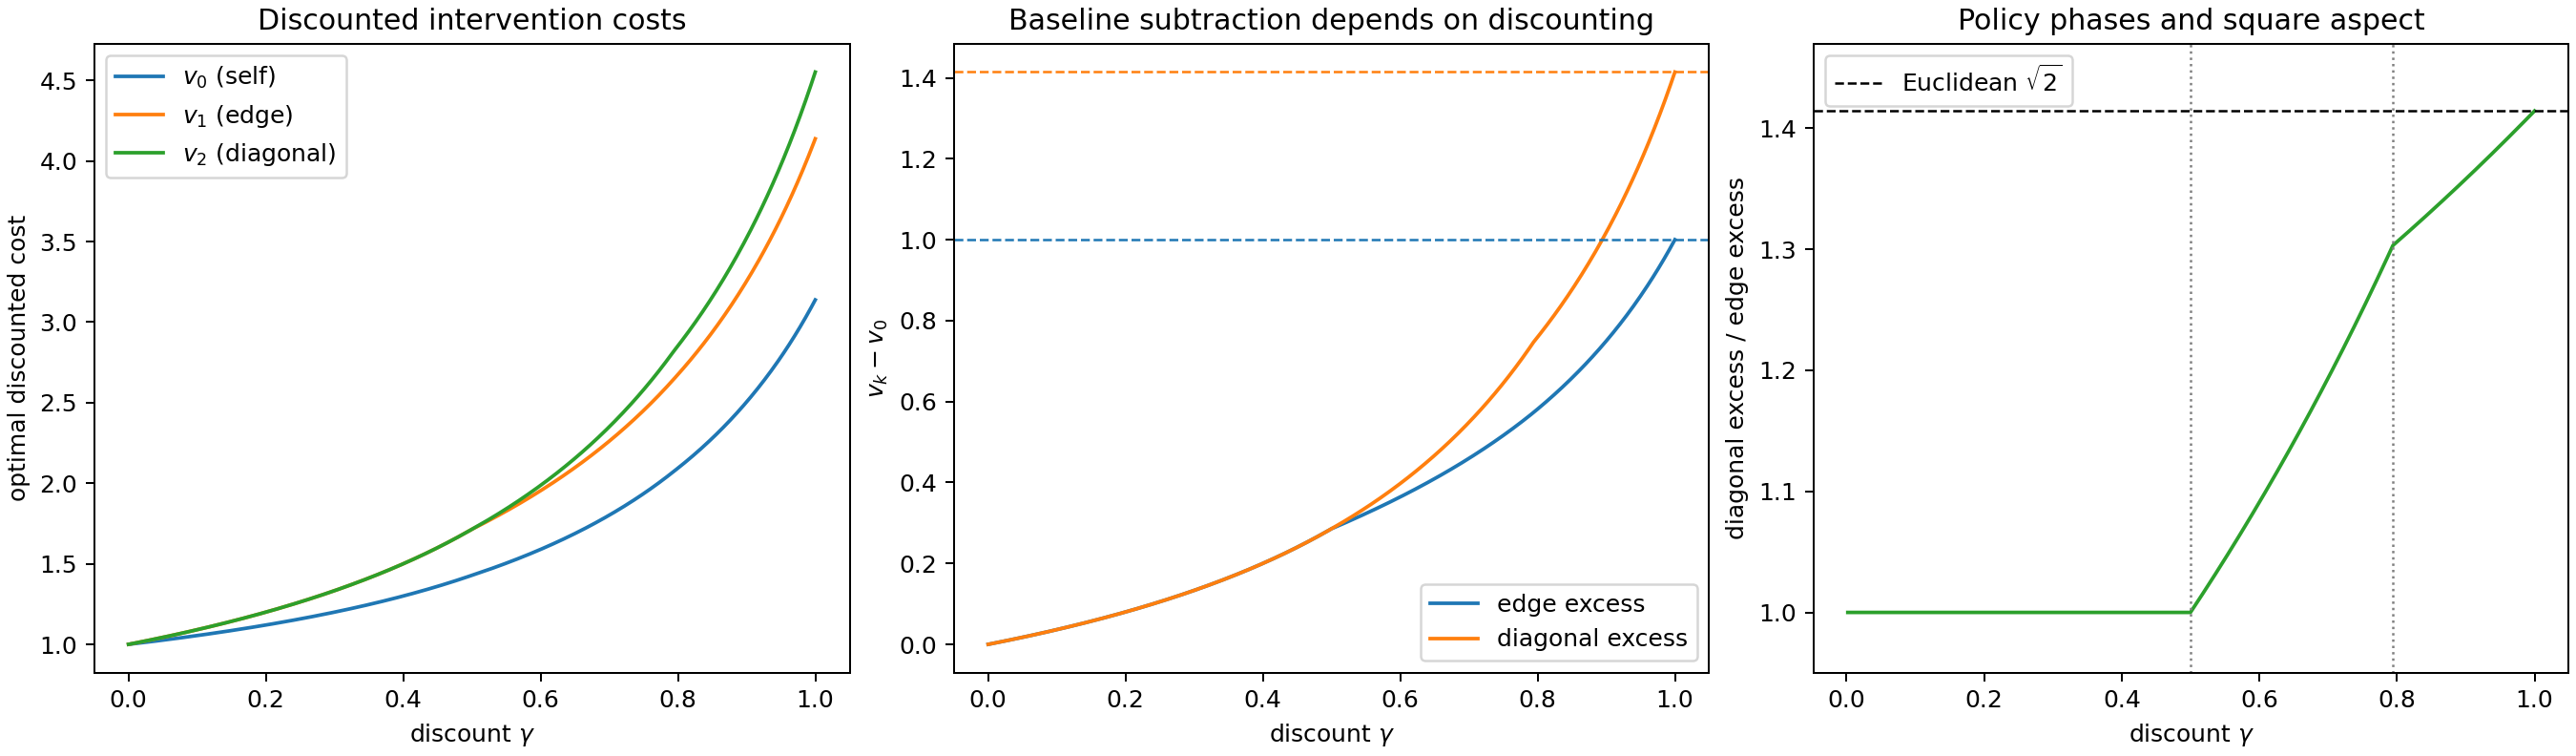
\includegraphics[width=\textwidth]{sic_discounting.png}
\caption{\textbf{Discounting changes both value and geometry.} Left: exact
discounted self, edge, and diagonal intervention costs. Center: after
subtracting the self reporting baseline, the edge and diagonal separations
reach \(1\) and \(\sqrt2\) only at \(\gamma=1\). Right: the diagonal-to-edge
ratio and the two exact policy thresholds \(\gamma=1/2\) and
\(\gamma=\gamma_*\). Strong discounting makes all non-goal SIC-report policies
optimal and collapses edge and diagonal into one shell.}
\label{fig:sic-discounting}
\end{figure}

\section{A compact derivation of the SIC reporting baseline}
\label{sec:reported-goal}

For reference, we can derive the common baseline in a compact three-shell
form. As specified in \cref{sec:complete-mdp}, goal \(g\) means: perform the
SIC action and observe outcome token \(g\). Every movement and every SIC report
costs one intervention. If a SIC outcome is not \(g\), the episode continues
from the newly prepared state \(\Pi_o\). After the first SIC outcome this is a
fully observed finite MDP, because the most recent token is a sufficient
operational state.

By square symmetry, write \(v_0,v_1,v_2\) for optimal cost when the current
anchor is respectively the goal, an axial neighbor, or the opposite corner.
The proposed policy reports at the goal, moves deterministically from an edge
to the goal, and retries the diagonal displacement from the opposite corner.
The two movement rules give
\begin{equation}
 v_1=1+v_0,
 \qquad
 v_2=\sqrt2+v_0.
 \label{eq:sic-shell-moves}
\end{equation}
At the goal state, the SIC reports \(g\) with probability \(1/2\), terminating
the episode. Its two edge outcomes have total probability \(1/3\), and its
diagonal outcome has probability \(1/6\). Consequently
\begin{align}
 v_0
 &=1+\frac13v_1+\frac16v_2\\
 &=1+\frac13(v_0+1)+\frac16(v_0+\sqrt2),
\end{align}
so
\begin{equation}
 \boxed{v_0=c:=\frac{8+\sqrt2}{3}}.
 \label{eq:sic-baseline}
\end{equation}
It follows that the full reported-goal value matrix is
\begin{equation}
 \boxed{V_g(x)=c+D(x,g).}
 \label{eq:sic-value}
\end{equation}

The remaining Bellman inequalities confirm optimality. At the goal, moving
first costs \(c+2>c\). At an edge, reporting immediately costs
\[
 1+\frac23v_1+\frac16v_2>v_1,
\]
while the axial move attains \(v_1\). At the diagonal, reporting costs
\[
 1+\frac13v_1+\frac12v_2>v_2,
\]
and an axial two-step route costs \(c+2>c+\sqrt2\); diagonal retry attains
\(v_2\). Thus \eqref{eq:sic-value} is the optimal Bellman solution, not merely
the value of a selected policy.

The nonzero self-value \(V_g(g)=c\) is the common overhead of requesting a
stochastic SIC report. Hodological separation is obtained by subtracting this
goal-specific self baseline:
\begin{equation}
 V_g(x)-V_g(g)=D(x,g).
 \label{eq:baseline-subtraction}
\end{equation}
The exact Euclidean square therefore survives when places and goals are both
defined entirely by experienced SIC outcomes.

Before the first SIC action, an agent with an unknown preparation occupies an
epistemic initial condition rather than one of four known anchors. Its first
SIC outcome both reports a token and prepares the associated state. Subsequent
tracking uses only that token, chosen actions, and observed success/failure
events; the policy needs no concealed binary-coordinate variable.

\section{Exact computation and finite-sample simulation}

The companion program \texttt{sic\_anchored\_square.py} constructs all density
matrices and Kraus operators, solves the four stochastic-shortest-path
problems, runs Monte Carlo navigation, and learns randomly renamed Pauli
permutations from anchor--action--SIC experiments. Eight focused tests verify
Kraus completeness, branch preparation, the \(1/2,1/6\) response kernel, the
analytic Bellman solution, every undiscounted action value, the three
discounted policy regimes, and optimal-policy structure.

At seed 20260813, exact value iteration gives
\[
 \max_{x,g}|V_g(x)-c-D(x,g)|=2.58\times10^{-14},
\]
and baseline subtraction recovers \(D\) to \(9.10\times10^{-15}\). Across
50,000 Monte Carlo episodes for each of the 16 ordered pairs, maximum mean-cost
error is \(0.02831\). In 500 independent opaque-label trials per sample size,
the complete four-action response permutations are recovered in every trial
at 100 samples per anchor/action pair. Across a 503-point discount scan, the
closed forms in \cref{sec:discounting} agree with numerical Bellman iteration
to \(3.02\times10^{-14}\).

\begin{figure}[p]
\centering
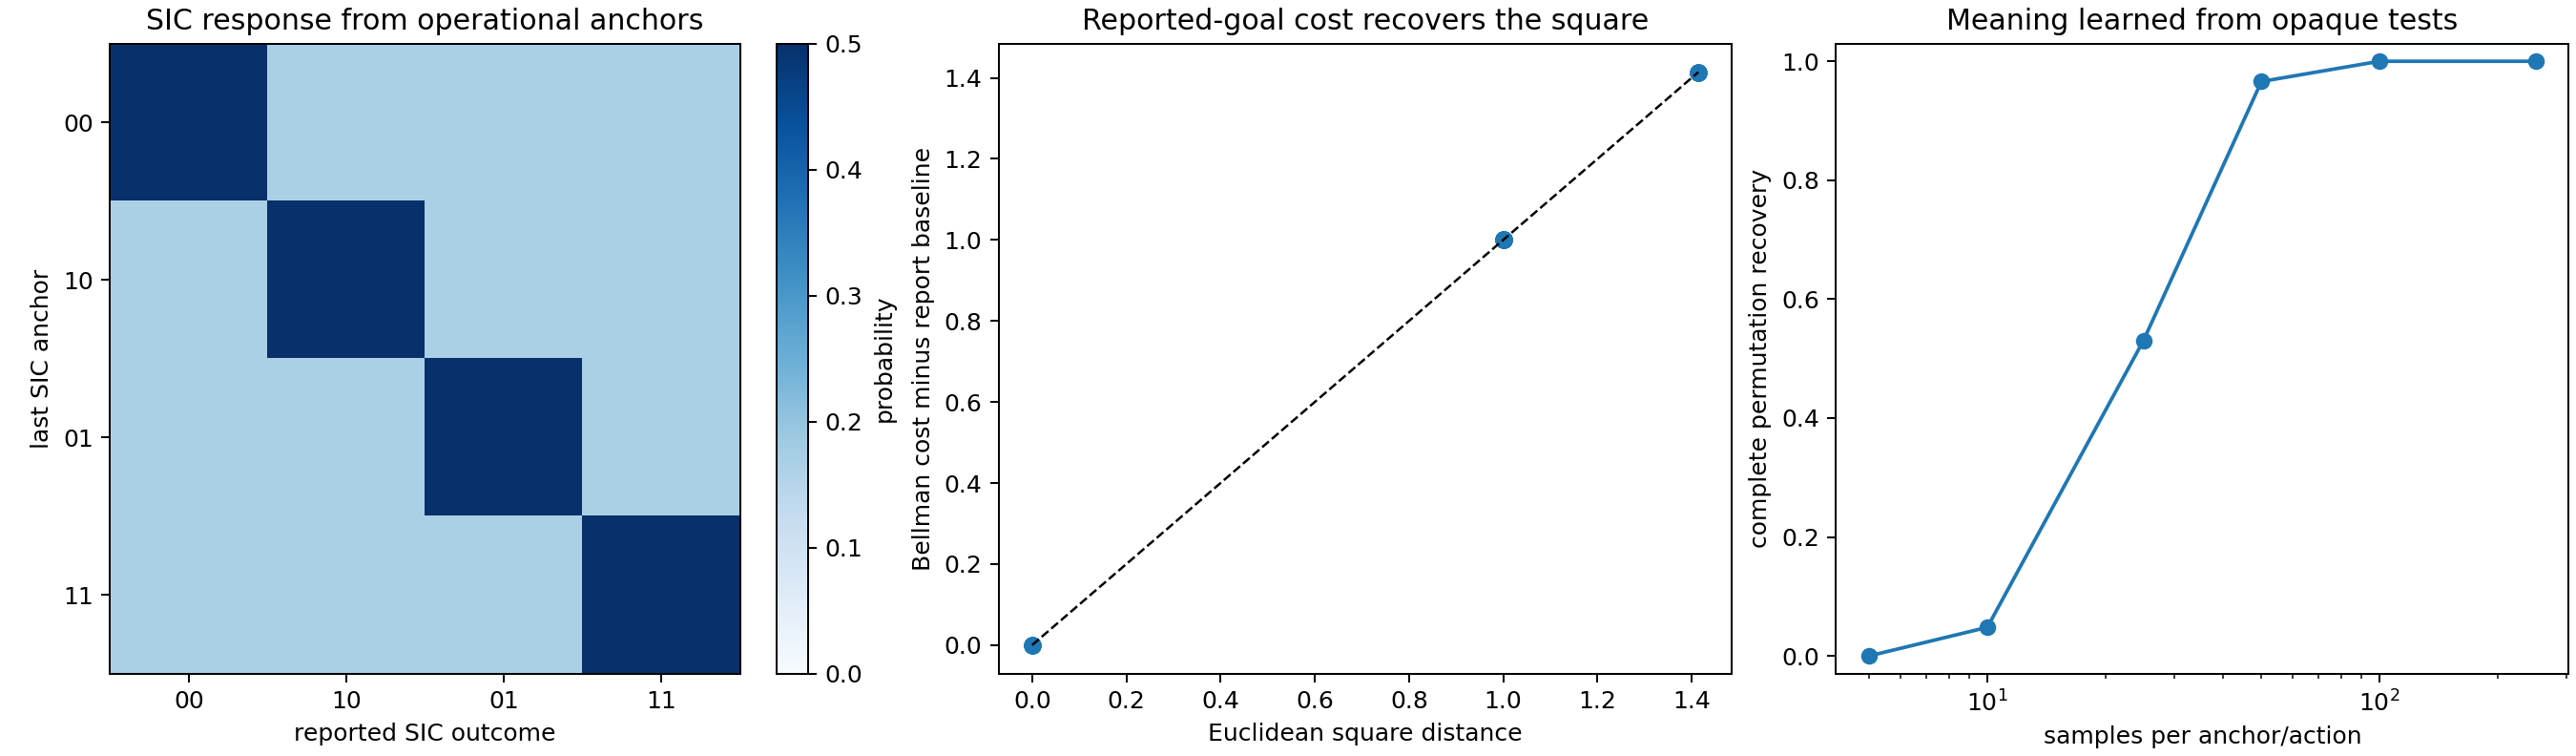
\includegraphics[width=\textwidth]{sic_anchored_square.png}
\caption{\textbf{The square grounded in SIC outcomes.} Left: after an observed
SIC anchor, the same outcome has probability \(1/2\), every other outcome has
probability \(1/6\), and every branch prepares the state named by its token.
Center: subtracting the common reporting baseline from exact Bellman costs
recovers side \(1\) and diagonal \(\sqrt2\). Right: randomly renamed Pauli
response permutations are learned from future SIC tests without exposing
binary coordinates.}
\label{fig:sic-anchored-square}
\end{figure}

\section{Why \(D\) is exactly a two-dimensional Euclidean metric}

The entries of \(D\) already match the familiar side and diagonal lengths of
a unit square.  Schoenberg's test certifies this without presupposing the
coordinates in \eqref{eq:coords}.

First square every entry:
\begin{equation}
 D^{\circ2}=\begin{pmatrix}
 0&1&1&2\\
 1&0&2&1\\
 1&2&0&1\\
 2&1&1&0
 \end{pmatrix}.
 \label{eq:D2}
\end{equation}
Every row mean, every column mean, and the grand mean of this matrix equal
one.  With
\[
 J=I-\frac14\bm1\bm1^T,
\]
the double-centered Gram matrix is
\begin{align}
 B&=-\frac12JD^{\circ2}J\\
 &=\begin{pmatrix}
 \frac12&0&0&-\frac12\\
 0&\frac12&-\frac12&0\\
 0&-\frac12&\frac12&0\\
 -\frac12&0&0&\frac12
 \end{pmatrix}.
 \label{eq:B}
\end{align}

To see the geometry directly, center the square coordinates:
\begin{equation}
 X=\begin{pmatrix}
 -\frac12&-\frac12\\
  \frac12&-\frac12\\
 -\frac12& \frac12\\
  \frac12& \frac12
 \end{pmatrix}.
 \label{eq:X}
\end{equation}
Multiplication gives \(XX^T=B\). Therefore \(B\) is positive semidefinite.
The two columns of \(X\) are orthonormal, so the eigenvalues of \(B\) are
\[
  1,\ 1,\ 0,\ 0.
\]
It has rank two, and classical multidimensional scaling reconstructs the four
rows of \(X\), up to rotation and reflection. This proves intrinsically that
the hodological metric \eqref{eq:D} is an exact two-dimensional Euclidean
metric.

\section{What the theorem proves---and what it assumes}

The theorem proves three useful facts.
\begin{enumerate}
\item The Kraus operators form valid quantum instruments.
\item The desired metric is achieved by a concrete policy.
\item The triangle inequality is a global certificate against every adaptive
shortcut.
\end{enumerate}

It does not derive the metric from an otherwise neutral quantum dynamics.  The
desired length is inserted into the success law \(p_h=1/d_G(\id,h)\). In the
square, the Euclidean diagonal is obtained because the diagonal action was
assigned success probability \(1/\sqrt2\). A different probability would
produce a different hodological diagonal.

It also does not imply that instrument outcomes localize the agent.  In a
random-unitary retry action, success/failure reports whether a chosen
translation occurred; it need not reveal the starting state.  Finally, the
four qubit states form a tetrahedron in Bloch-state geometry even though their
optimal costs form a square.  This separation is intentional: hodological
distance measures difficulty of controlled goal achievement, not quantum
state overlap.

The SIC extension in \cref{sec:sic-anchor,sec:reported-goal} repairs the
location-token problem in a precise sense: an outcome prepares and therefore
identifies the \emph{postmeasurement} anchor, and place goals are future SIC
outcomes. It does not retrospectively identify the unknown premeasurement
state, nor make the retry movement outcome itself location-informative. Its
virtue is that the agent's current-state token and its goal tokens now arise
from one actual measurement alphabet.

\section{A compact checklist for using the theorem}

Before applying the retry theorem to a new construction, check:
\begin{enumerate}
\item Is every desired displacement represented by a valid group element?
\item Is the orbit faithful after quotienting global phase and the fiducial
stabilizer?
\item Does the side of multiplication match the side of metric invariance?
\item Has the metric been normalized so every \(p_h\le1\)?
\item Does failure truly leave the operational coordinate unchanged?
\item Is the goal defined by the physical orbit, a predictive equivalence
class, or an external group-product monitor?  These are not interchangeable.
\item Is \(p_h=1/d_G(\id,h)\) physically motivated, learned, or simply supplied
by design?
\end{enumerate}

For Eq.~(43), all algebraic conditions hold exactly.  The remaining scientific
limitation is the last one: the Euclidean success law is engineered rather
than derived.

\end{document}
